\documentclass{article}
%%%%%%%%%%%%%%%%%%%%%%%%%%%%%%%%%%%%%%%%%%%%%%%%%%%%%%%%%%%
%% package sillabazione italiana e uso lettere accentate
\usepackage[latin1]{inputenc}
\usepackage[english]{babel}
\usepackage[T1]{fontenc}
%%%%%%%%%%%%%%%%%%%%%%%%%%%%%%%%%%%%%%%%%%%%%%%%%%%%%%%%%%%%%

\usepackage{url}
\usepackage{xspace}
\usepackage{listings}
\usepackage{xcolor}

\usepackage[top=1in, bottom=1in, left=1in, right=1in]{geometry}

\makeatletter
%%%%%%%%%%%%%%%%%%%%%%%%%%%%%% User specified LaTeX commands.
\usepackage{manifest}

\makeatother

%%%%%%%
 \newif\ifpdf
 \ifx\pdfoutput\undefined
 \pdffalse % we are not running PDFLaTeX
 \else
 \pdfoutput=1 % we are running PDFLaTeX
 \pdftrue
 \fi
%%%%%%%
 \ifpdf
 \usepackage[pdftex]{graphicx}
 \else
 \usepackage{graphicx}
 \fi
%%%%%%%%%%%%%%%
 \ifpdf
 \DeclareGraphicsExtensions{.pdf, .jpg, .tif}
 \else
 \DeclareGraphicsExtensions{.eps, .jpg}
 \fi
%%%%%%%%%%%%%%%

\newcommand{\java}{\textsf{Java}}
\newcommand{\contact}{\emph{Contact}}
\newcommand{\corecl}{\texttt{corecl}}
\newcommand{\medcl}{\texttt{medcl}}
\newcommand{\msgcl}{\texttt{msgcl}}
\newcommand{\android}{\texttt{Android}}
\newcommand{\dsl}{\texttt{DSL}}
\newcommand{\jazz}{\texttt{Jazz}}
\newcommand{\rtc}{\texttt{RTC}}
\newcommand{\ide}{\texttt{Contact-ide}}
\newcommand{\xtext}{\texttt{XText}}
\newcommand{\xpand}{\texttt{Xpand}}
\newcommand{\xtend}{\texttt{Xtend}}
\newcommand{\pojo}{\texttt{POJO}}
\newcommand{\junit}{\texttt{JUnit}}

\newcommand{\action}[1]{\texttt{#1}\xspace}
\newcommand{\code}[1]{{\small{\texttt{#1}}}\xspace}
\newcommand{\codescript}[1]{{\scriptsize{\texttt{#1}}}\xspace}

% Cross-referencing
\newcommand{\labelsec}[1]{\label{sec:#1}}
\newcommand{\xs}[1]{\sectionname~\ref{sec:#1}}
\newcommand{\xsp}[1]{\sectionname~\ref{sec:#1} \onpagename~\pageref{sec:#1}}
\newcommand{\labelssec}[1]{\label{ssec:#1}}
\newcommand{\xss}[1]{\subsectionname~\ref{ssec:#1}}
\newcommand{\xssp}[1]{\subsectionname~\ref{ssec:#1} \onpagename~\pageref{ssec:#1}}
\newcommand{\labelsssec}[1]{\label{sssec:#1}}
\newcommand{\xsss}[1]{\subsectionname~\ref{sssec:#1}}
\newcommand{\xsssp}[1]{\subsectionname~\ref{sssec:#1} \onpagename~\pageref{sssec:#1}}
\newcommand{\labelfig}[1]{\label{fig:#1}}
\newcommand{\xf}[1]{\figurename~\ref{fig:#1}}
\newcommand{\xfp}[1]{\figurename~\ref{fig:#1} \onpagename~\pageref{fig:#1}}
\newcommand{\labeltab}[1]{\label{tab:#1}}
\newcommand{\xt}[1]{\tablename~\ref{tab:#1}}
\newcommand{\xtp}[1]{\tablename~\ref{tab:#1} \onpagename~\pageref{tab:#1}}
% Category Names
\newcommand{\sectionname}{Section}
\newcommand{\subsectionname}{Subsection}
\newcommand{\sectionsname}{Sections}
\newcommand{\subsectionsname}{Subsections}
\newcommand{\secname}{\sectionname}
\newcommand{\ssecname}{\subsectionname}
\newcommand{\secsname}{\sectionsname}
\newcommand{\ssecsname}{\subsectionsname}
\newcommand{\onpagename}{on page}

\newcommand{\xauthA}{Roberto Casadei }
\newcommand{\xauthB}{Massimiliano Martella}
\newcommand{\xauthC}{Roberto Reda}
\newcommand{\xfaculty}{II Faculty of Engineering}
\newcommand{\xunibo}{Alma Mater Studiorum -- University of Bologna}
\newcommand{\xaddrBO}{viale Risorgimento 2}
\newcommand{\xaddrCE}{via Venezia 52}
\newcommand{\xcityBO}{40136 Bologna, Italy}
\newcommand{\xcityCE}{47023 Cesena, Italy}

\usepackage{float}

%
% Comments
%
%%% \newcommand{\todo}[1]{\bf{TODO:}\emph{#1}}


\begin{document}

\title{Software Systems Engineering\\
 process report template}

%%% \author{\xauthA \and \xauthB}
\author{\xauthA \and \xauthB \and \xauthC}


%\institute{%
%%%  \xunibo\\\xaddrCE, \xcityCE\\\email{\{nameA.studentA, nameB.studentB\}@studio.unibo.it}
%  \xunibo\\\xaddrCE, \xcityCE\\\email\ roberto.casadei12@studio.unibo.it
%}

\maketitle

%% \begin{abstract}
%% \footnotesize
%%This a Latex template to be used for the reports of Software Engineering.
%%\keywords{Software engineering, managed software development, reports, ....}
%%\end{abstract}

%%% \sloppy

%===========================================================================
\section{Introduction}
\labelsec{intro}
%===========================================================================

 This report represents a snapshot of the current status 
  of the ``ButtonLed'' project (object-based).

%===========================================================================
\section{Vision}
\labelsec{Vision}
%===========================================================================

We believe that a good software product is the natural result of a
\textbf{mature, systematic process}.

\emph{We believe that there is no code without design, no design without
analysis, no analysis without requirements.} So, we recognize the causal
progression from the \emph{why} (vision/goals/requirements) to the \emph{what}
(analysis) and finally to the \emph{how} (design/code).

We recognize the importance of analysis for a mature process, but we don't want
to waste time by just producing informal knowledge. Instead, we would like to \textbf{capitalize the
effort spent in analysis by producing something that has value, that is, working software (prototype) and reusable frameworks}.
That is, we believe that \emph{reuse} is prominent in what we do.

We also think that following a \textbf{top-down approach}, i.e., from the
problem to the technology, is extremely valuable because it can adequately
support our goals. In doing so, we would like to constantly \textbf{evaluate the
abstraction gap} in order to gain a better vision of what we need to
\emph{effectively} build the kind of systems we are considering and also as a
way to \emph{innovate}.

Moreover, as we are dealing with (complex) software systems, we believe
that a \textbf{systemic approach} fits more than an algorithmic approach and 
gives us access to more powerful conceptual tools.

Last but not least, we think that a software development process built upon the
principles outlined above can maximize the value of the effort spent
during analysis and development, effectively produce software architectures that
are resistant to requirements change, and even turn those changes into an
opportunity to increase the organizational know-how.

% TRACEABILITY

% WHY -> WHAT -> HOW

%===========================================================================
\section{Goals}
\labelsec{Goals}
%===========================================================================

 We use the ButtonLed system as an opportunity to actualize the vision. The
 ButtonLed system, in its simplicity, captures the essential characteristics of
 all the software systems: input, elaboration, output. In this case study, the
 technology hypothesis is given by the object-oriented paradigm.\\

We are aware that the system we are building is just one of the countless
applications that could be built in this domain. So, we generalise/abstract from
the issues we encounter in a sustainable manner, so that we can \textbf{factor
domain-knowledge out of the specific system}.

Also, by analyzing the requirements and the problem, we would like to produce a
\textbf{working prototype by following an incremental (\emph{piecemeal growth})
approach}.

In particular, we would like to evaluate the cost of passing from a homogeneous,
concentrated system to a distributed, etherogeneous system.

Moreover, we would like to correlate what we do with the following concepts:

\begin{itemize}
  \item Models ($\Rightarrow$ Structure, Interaction, Behavior) as a way to
  capture the essential characteristics of what we talk about
  \item Software reuse as the key element to deal with bounded resources
     \begin{itemize}
       \item Design patterns as synthetic analyses and design ideas for
       recurring problems
       \item Framework vs. pattern vs. middleware
	 \end{itemize}
  \item Technologies as specific ways to actualize designs but also as
  conceptual spaces (i.e., ``representing'' a paradigm)
  \item Logic architecture as the main result from analysis and possibly our
  main specification of the problem at hand
  \item Traceability (from requirements to architecture to code) as a way to
  support ``informational consistency'' within the project
  \item Specific vs. schematic vs. generic parts of software
\end{itemize}



%===========================================================================
\section{Requirements}
\labelsec{Requirements}
%===========================================================================

\begin{quote}''
Design and build a ButtonLed software system in which a Led is turned on and off
each time a Button is pressed.
In particular, the system will have the button on an Android device, 
 the controller on a RaspberryPi, and the led on Arduino.
``\end{quote}

 
%===========================================================================
\section{Requirement analysis}
\labelsec{ReqAnalysis}
%===========================================================================

From the requirements, it follows that the system is structurally composed of
(at least) three \textbf{subsystems} (for which we already know the deployment,
see the Deployment section \ref{sec:Deployment}):
 
\begin{itemize}
  \item One subsystem (on Android) with the button
  \item One subsystem (on Raspberry) with the controller
  \item One subsystem (on Arduino) with the led
\end{itemize}

It also follows that \textbf{distribution} and \textbf{etherogeneity} are
essential characteristics of the system.

As noted above, three main entities arise from the requirements: the button,
the controller, and the led.

Note that the controller is explicitly considered in the current version of the
requirements. However, in the last \emph{iteration}, the notion of a controller
resulted from the problem analysis, as we noted that the responsibility of
``notiying the led when the button is pressed'' could NOT be assigned to the
button, nor to the led.


\subsection{Use cases}
\labelssec{UseCases}

\begin{figure}[H]
    \centering
     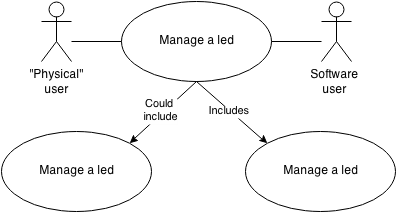
\includegraphics[scale = 0.6]{img/BLS-UseCase.png}
    \caption{Use case 1}
    \label{fig:usecase1}
\end{figure}


\subsection{Scenarios}
\labelssec{Scenarios}

 (Skipped) It's not a primary goal of this case study.

\subsection{(Domain)model}



From the requirements we know that:

\begin{itemize}
  \item The button has a state (pressed
  and not pressed) and, as external entities are interested in that state, it
  follows that it should be an \emph{observable} entity (see the
  \emph{Observer} pattern)
  \item The led has a state as well (on, off) and properties such as the color.
\end{itemize}

The requirements explicitly give information about the structure of the system
and the components, and express a cause-effect relationship between the press of
the button and the update of the state of the led. Instead, the dimensions of
behavior and interaction are only implictly and partially described by an
\emph{observational} point of view.	\\
 
To explain what we mean by ``led" and ``button", we provide a \textbf{model} for
them.

By following an internal convention, we express those models using Java
\textbf{interfaces}. As interfaces are not sufficient, we also provide
\textbf{test plans} in order to better define our intended semantics.
 
By analyzing our idea of ``button" and ``led", we also note that, in the domain
of the \emph{Internet of Things}, the led and the button are particular
instance of the concept of \textbf{device}. Moreover, we know that a
particular device can be realized (implemented) with different technologies
(see the \emph{Bridge pattern})

\lstset{frame=single, language=java, breaklines=true, numbers=left,
basicstyle=\fontfamily{pcr}\selectfont\footnotesize\color{black},
    keywordstyle=\color{blue}\bfseries,}
    
  \lstinputlisting[caption=it.unibo.buttonLed.interfaces.IDevice]
  {../it.unibo.group08.interfaces/src/it/unibo/buttonLed/interfaces/IDevice.java}    
  
  \lstinputlisting[caption=it.unibo.buttonLed.interfaces.IDeviceInput]
  {../it.unibo.group08.interfaces/src/it/unibo/buttonLed/interfaces/IDeviceInput.java}    
        
  \lstinputlisting[caption=it.unibo.buttonLed.interfaces.ILed]
  {../it.unibo.group08.interfaces/src/it/unibo/buttonLed/interfaces/ILed.java}

  \lstinputlisting[caption=it.unibo.buttonLed.interfaces.IButton]
  {../it.unibo.group08.interfaces/src/it/unibo/buttonLed/interfaces/IButton.java}


\subsubsection{Behavior}\\

\begin{figure}[H]
    \centering
     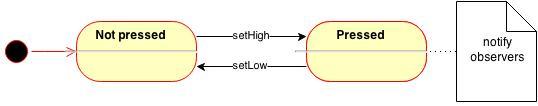
\includegraphics[scale=0.65]{img/ISS-FSM-Button.png}
    \caption{Button: behavior}
\end{figure}

\begin{figure}[H]
    \centering
     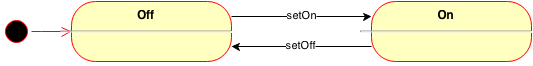
\includegraphics[scale=0.65]{img/ISS-FSM-Led.png}
    \caption{Led: behavior}
\end{figure}


\subsection{Test plan}

 See \emph{it.unibo.group08.buttonled.test} project.

%===========================================================================
\section{Problem analysis}
\labelsec{ProblemAnalysis}
%===========================================================================


\subsection{Logic architecture}

The system is composed of three main components: the led, the button, and the
controller.

From the requirements, we also know that they are on different subsystems (see
Requirements Analysis in Section \ref{sec:ReqAnalysis}).


\begin{figure}[H]
    \centering
     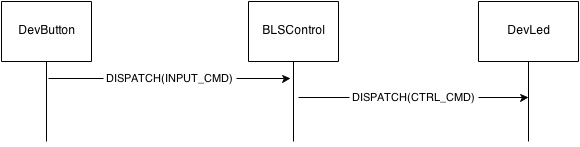
\includegraphics[scale=0.75]{img/BLSLogicalArch.png}
    \caption{Logic Architecture -- Structure/Interaction view}
    \label{fig:logicarch_inter}
\end{figure}

Please consult the software house's internal reference to get a description of
the semantics of the ``DISPATCH'' message.

For simplicity, at the moment we can think at the communication language as
described by the following grammar:

\begin{lstlisting}
INPUT_CMD = 0 | 1
CTRL_CMD = 0 | 1
\end{lstlisting}

The controller's behavior can be represented by the following FSM:

\begin{figure}[H]
    \centering
     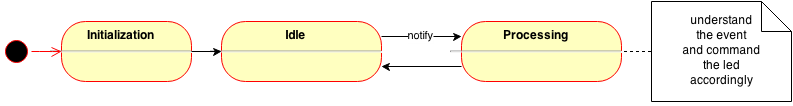
\includegraphics[scale=0.65]{img/ISS-FSM-Controller.png}
    \caption{Controller: behavior}
\end{figure}



\subsection{Abstraction gap}

Our technology hypothesis is given by the object-oriented paradigm 
 (and, in practice, by Java).

The problem and the practical issues encountered through the analysis phase
point out that a gap exists with respect to the following themes/areas:

\begin{itemize}
  \item \textbf{Model specification}: we have specified the models of the
  system and the components using Java interfaces, test plans, and (custom
  variants of) UML.
  However, our need of producing models that are both formal and expressed at the right
  level of abstraction is not adequately satisfied.
  
  \item \textbf{``General'' system concepts}: OOPLs do not (directly)
  support our system view (which we use instead of an algorithmic view) through
  high-level concept such as ``environment'', ``situated entity'', ``named
  entity'', \ldots $\Rightarrow$ our effort in filling this gap has resulted in
  the \emph{it.unibo.system} package (within \emph{it.unibo.noawtsupports})
  
  \item \textbf{Rapid prototyping}: our goal to have analysis end up with a
  (graphical) prototype is not effectively supported by Java GUI libraries
  (AWT, Swing) $\Rightarrow$ our effort in filling this gap has resulted in
  \emph{it.unibo.envBaseAwt}
  
  \item \textbf{Communication infrastructure}: in this technology hypothesis,
  the communications between the system's components are not adequately
  supported $\Rightarrow$ the need to delegate the technology-specific details of
  communications to the infrastructure brought our software house to develop
  \emph{it.unibo.noawtsupports}
  
  \item \textbf{Interaction semantics}: the high-level semantics of the
  interaction between the system's components is not directly captured by neither the tools we use
  to express models nor by our platform.  We conventionally
  introduced some names (dispatch, request, signal, \ldots) to
  specify a vocabulary for (informally) talking about interaction at the level
  of abstraction we consider more appropriate. However, this semantics is not
  directly supported.
\end{itemize}
 
In particular, we note that the issue of ``distribution'' generates forces that
urge us to consider a message-passing style for
interaction.

\subsection{Risk analysis}

  If we don't adequately fill the abstraction gap, and if we don't abstract
  from technology-specific and application-specific details, we risk to have
  significant losses in case of change of (both functional and non-functional) requirements.
  

%===========================================================================
\section{Work plan}
\labelsec{wplan}
%===========================================================================

The project team consists of three engineers. So, ideally, the work is
subdivided on a subsystem-basis:

\begin{itemize}
  \item One developer will design/develop the Android subsystem
  \item One developer will design/develop the RaspberryPi subsystem
  \item One developer will design/develop the Arduino subsystem
\end{itemize}

Here, it is important to clearly define the subsystems' interfaces
(communication media, communication language, \ldots). An architectural design
will be defined (see Section \ref{sec:Project}) to better specify the
constraints and interactions.

Moreover, certain code/naming conventions should be defined in order to preserve
the internal quality (coherence) of the system.

%===========================================================================
\section{Project}
\labelsec{Project}
%===========================================================================

\begin{figure}[H]
    \centering
     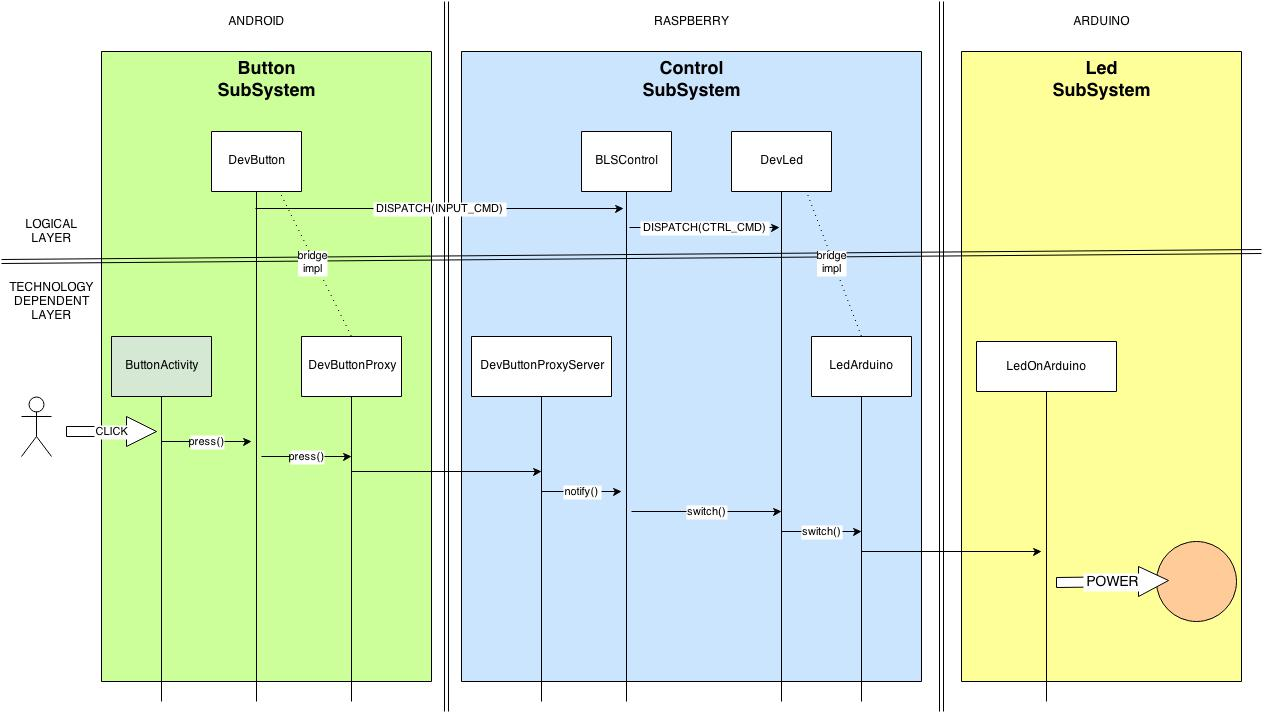
\includegraphics[scale=0.42]{img/BLS-FullDistribHetherogeneousV2.jpg}
    \caption{Design architecture}
    \label{fig:designarch}
\end{figure}


Notes:

\begin{itemize}
  \item The pattern \emph{Proxy} is used to hide the details of network-based
  communication when requesting operations to the button/led/controller
\end{itemize}

%\subsection{Structure}
%\subsection{Interaction}
%\subsection{Behavior}

%===========================================================================
\section{Implementation}
\labelsec{Implementation}
%===========================================================================

 See \emph{it.unibo.group08.buttonled.logical} and 
 \emph{it.unibo.group08.buttonled.system} projects.

%===========================================================================
\section{Testing}
\labelsec{testing}
%===========================================================================

 See \emph{it.unibo.group08.buttonled.test} project.

%===========================================================================
\section{Deployment}
\labelsec{Deployment}
%===========================================================================

 Directly from the requirements, the following deployment configuration follows:
 
 \begin{itemize}
   \item An APK package for the Android subsystem
   \item A JAR package for the RaspberryPi subsystem
   \item A INO file for the Arduino subsystem
 \end{itemize}

%===========================================================================
\section{Maintenance}
\labelsec{Maintenance}
%===========================================================================

%\newpage
%See \cite{natMol09} until page 11 (\texttt{CMM}) and pages 96-105.

%===========================================================================
\section{Information about the authors}
\labelsec{Author}
%===========================================================================

\vskip.5cm
%%% \begin{figure}
\begin{tabular}{ | c | c | c |  }
\hline
  % after \\: \hline or \cline{col1-col2} \cline{col3-col4} ...
   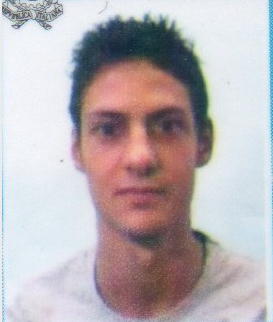
\includegraphics[scale = 0.4]{img/fototessera.jpg}
   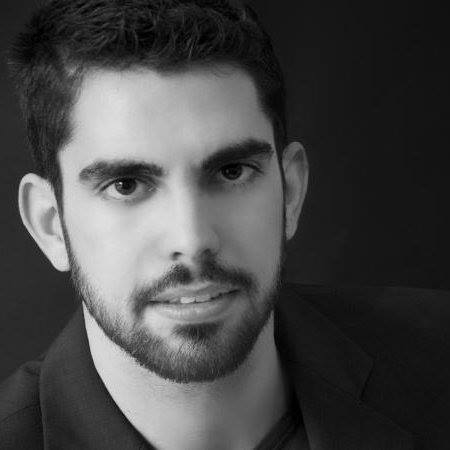
\includegraphics[scale = 0.25]{img/reda.jpg}
   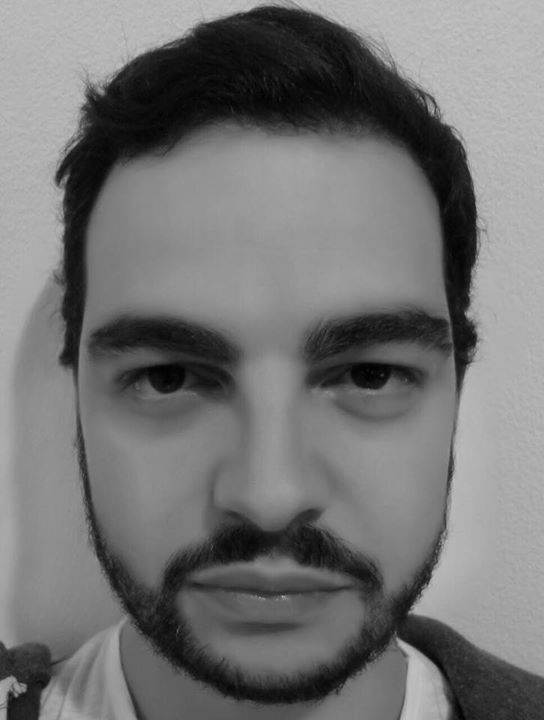
\includegraphics[scale = 0.18]{img/martella.jpg}
\end{tabular}


%%% \begin{itemize}
%%% \item Titolo di studio:\\ \\
%%% \item Interessi particolari:\\ \\
%%% \item Ha sostenuto fino ad oggi il seguente numero di esami:\\ \\
%%% \item Deve ancora sostenere i seguenti esami del I anno:\\ \\
%%% \item Prevede di svolgere un tirocinio presso:\\ \\
%%% \item Prevede di laurearsi nella sessione:\\ \\
%%% \item Intende proseguire gli studi per conseguire: \\  \\  \\
%%%   	presso la sede universitaria di: \\ \\
%%% \item Intende entrare subito nel mondo del lavoro presso : \\ \\
%%% \end{itemize}

 
\appendix

\nocite{gof94}
\bibliographystyle{abbrv}
\bibliography{biblio}

\end{document}












